\section{NonLinear}
\subsection{Bisection Method}
\begin{algorithm}[H]
\SetAlgoLined
    \SetKwInOut{Input}{Input}
    \SetKwInOut{Output}{Output}
    \SetKwProg{Fn}{Function}{}{}
\Input{Function $f$, interval $[a,b]$, number of maximum iterations $stop\_iters$, argument list $*args$}
\Output{Approximate zero of $f$}
\Fn{bisect($fun, interval, stop\_iters, iters, *args$)}{
  $x_0, x_1 \gets a, b$ \;
  $f_0, f_1 \gets f(x_0,*args), f(x_1,*args)$ \;
  \If{$f_0 \times f_1 > 0$}{
    \textbf{raise} ValueError("No zeros in the given interval") \;
  }
  $x \gets x_1$ \;
  $iterations \gets 0$ \;
  \While{$f_1 \neq 0$ \textbf{and} $iterations < stop\_iters$}{
    $iterations \gets iterations + 1$ \;
    $x \gets 0.5 \cdot (x_0 + x_1)$ \;
    $f \gets f(x, *args)$ \;
    \If{$f \times f_1 < 0$}{
      $x_0 \gets x$ \;
    } \Else{
      $x_1 \gets x$ \;
      $f_1 \gets f$ \;
    }
  }
  \If{iters}{
    \KwRet{$x, iterations$} \;
  }
  \KwRet{$x$} \;
  }
  \caption{Bisection Method}
\end{algorithm}
\subsubsection{BNumMet Examples}
\paragraph{Example 1}{
\begin{lstlisting}[language=Python]
from BNumMet.NonLinear import bisect
fun = lambda x: x**2 - 2
interval = [1, 2]
sol, nIter = bisect(fun, interval, iters = True)
print("Bisection method: x = %f, nIter = %d" % (sol, nIter))

>> Bisection method: x = 1.414214, nIter = 100
\end{lstlisting}
}
\paragraph{Example 2}{
\begin{lstlisting}[language=Python]
from BNumMet.NonLinear import bisect
f = lambda x: sp.jv(0, x) # Bessel function of the first kind of order 0
interval = lambda n: [n * np.pi, (n + 1) * np.pi] # Interval for the n-th zero

zeros = [ bisect(f, interval(n)) for n in range(0, 10)]


x = np.arange(1, 10 * np.pi, np.pi / 50)
y = f(x)
plt.plot(x, y)
plt.plot(zeros, np.zeros(len(zeros)), "ro")
plt.axhline(0, color="k")
plt.show()
\end{lstlisting}
\begin{figure}[H]
    \centering
    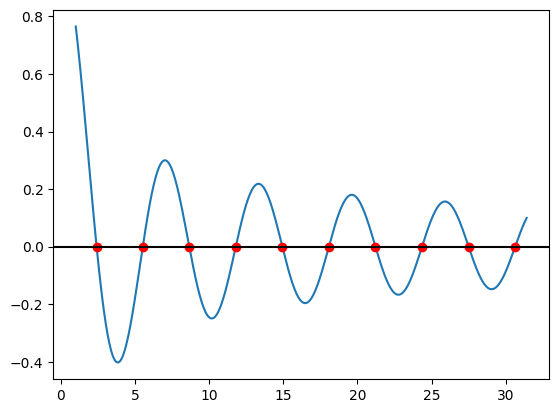
\includegraphics{Include/Images/Thesis/Documentation/NonLinear/Bisect Example 2.png}
    \caption{Bisect Example 2}
    \label{fig:Bisect Example 2}
\end{figure}
}



\subsection{Secant Method}
\begin{algorithm}[H]
\SetAlgoLined
    \SetKwInOut{Input}{Input}
    \SetKwInOut{Output}{Output}
    \SetKwProg{Fn}{Function}{}{}
\Input{Function $f$, interval $[a,b]$, number of maximum iterations $stop\_iters$, argument list $*args$}
\Output{Approximate zero of $f$}
\Fn{secant($fun, interval, stop\_iters, iters, *args$)}{initialization: x0, x1 = interval\;
 f0 = fun(x0, *args)\;
 f1 = fun(x1, *args)\;
 \eIf{f0 * f1 > 0}{
  raise ValueError("The function has no zeros in the given interval")\;
  }{
   iterations = 0\;
   \While{abs(x1 - x0) > $\epsilon$ and iterations < stop\_iters}{
    iterations += 1\;
    x2 = x0\;
    x0 = x1\;
    x1 = x1 + (x1 - x2) / (fun(x2, *args) / fun(x1, *args) - 1)\;
   }
   \eIf{iters}{
    return x1, iterations\;
    }{
    return x1\;
   }
  }}
 \caption{Secant Method}
\end{algorithm}
\subsubsection{BNumMet Examples}
\paragraph{Example 1}{
\begin{lstlisting}[language=Python]
from BNumMet.NonLinear import secant
fun = lambda x: x**2 - 2
interval = [1, 2]
sol, nIter = secant(fun, interval, iters = True)
print("Secant method: x = %f, nIter = %d" % (sol, nIter))

>> Secant method: x = 1.414214, nIter = 7
\end{lstlisting}
}
\paragraph{Example 2}{
\begin{lstlisting}[language=Python]
f = lambda x: sp.jv(0, x) # Bessel function of the first kind of order 0
interval = lambda n: [n * np.pi, (n + 1) * np.pi] # Interval for the n-th zero

zeros = [ secant(f, interval(n)) for n in range(0, 10)]


x = np.arange(1, 10 * np.pi, np.pi / 50)
y = f(x)
plt.plot(x, y)
plt.plot(zeros, np.zeros(len(zeros)), "ro")
plt.axhline(0, color="k")
plt.show()
\end{lstlisting}
\begin{figure}[H]
    \centering
    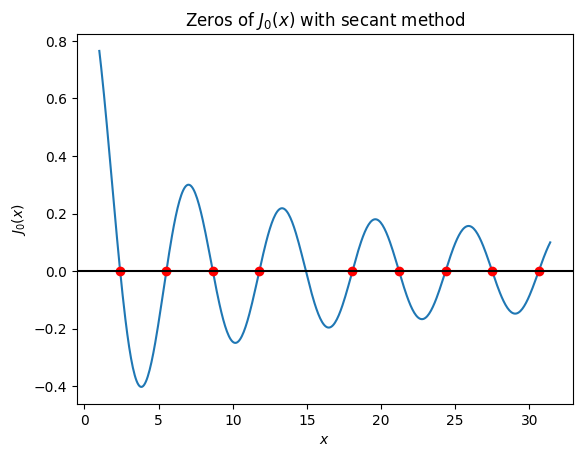
\includegraphics{Include/Images/Thesis/Documentation/NonLinear/Secant Example 2.png}
    \caption{Secant Example 2}
    \label{fig:Secant Example 2}
\end{figure}
}

\subsection{Newton's Method}
\begin{algorithm}[H]
\SetAlgoLined
    \SetKwInOut{Input}{Input}
    \SetKwInOut{Output}{Output}
    \SetKwProg{Fn}{Function}{}{}
\Input{fun, derivative, start\_point, stop\_iters=100, iters=False, *args}
\Output{x: zeros of the function fun}
\Fn{newton($fun, derivative, start\_point, stop\_iters, iters, *args$)}
{ 
initialization: previous\_x = start\_point - 1\;
 xn = start\_point\;
 fn = fun(xn, *args)\;
 \eIf{derivative(xn, *args) == 0}{
  raise ValueError("The derivative of the function is zero")\;
  }{
   iterations = 0\;
   \While{fn != 0 and not np.isclose(xn - previous\_x, 0) and derivative(xn, *args) != 0 and iterations < stop\_iters}{
    iterations += 1\;
    previous\_x = xn\;
    xn = xn - fn / derivative(xn, *args)\;
    fn = fun(xn, *args)\;
   }
   \eIf{iters}{
    return xn, iterations\;
    }{
    return xn\;
   }
  }}
 \caption{Newton-Raphson Method}
\end{algorithm}
\subsubsection{BNumMet Examples}
\paragraph{Example 1}{
\begin{lstlisting}[language=Python]
from BNumMet.NonLinear import newton
fun = lambda x: x**2 - 2
derivative = lambda x: 2 * x
interval = [1, 2]
sol, nIter = newton(fun, derivative, start_point=2, iters = True)
print("Newton's method: x = %f, nIter = %d" % (sol, nIter))
\end{lstlisting}
}
\paragraph{Example 2}{
\begin{lstlisting}[language=Python]
f = lambda x: sp.jv(0, x) # Bessel function of the first kind of order 0
derivative = lambda x: sp.jvp(0, x, 1) # Derivative of the Bessel function
interval = lambda n: [n * np.pi, (n + 1) * np.pi] # Interval for the n-th zero

zeros = [ newton(f, derivative, start_point = interval(n)[0]) for n in range(1, 11)]


x = np.arange(1, 10 * np.pi, np.pi / 50)
y = f(x)
plt.plot(x, y)
plt.plot(zeros, np.zeros(len(zeros)), "ro")
plt.axhline(0, color="k")
plt.show()
\end{lstlisting}
}
\begin{figure}[H]
    \centering
    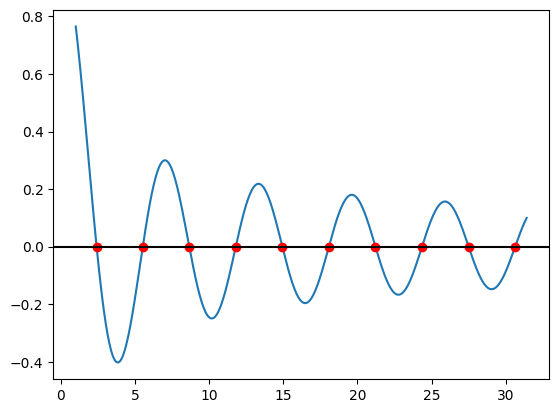
\includegraphics{Include/Images/Thesis/Documentation/NonLinear/Newtons Example 2.png}
    \caption{Newton's Method Example 2}
    \label{fig:Newton's Method Example 2}
\end{figure}
\subsection{Inverse Quadratic Interpolation (I.Q.I.)}
\begin{algorithm}[H]
\SetAlgoLined
    \SetKwInOut{Input}{Input}
    \SetKwInOut{Output}{Output}
    \SetKwProg{Fn}{Function}{}{}

    \Input{Function $f$, Initial values of $x_0$, $x_1$, $x_2$, Maximum number of iterations $stop\_iters$, and Optional arguments $args$}
    \Output{Zeros of the function $f$}
    \Fn{IQI($f, x\_values, stop\_iters, iters, *args$)}{
        $x_0, x_1, x_2 \leftarrow x\_values$\;
        $iterations \leftarrow 0$\;
        \While{$\left| x_1 - x_0 \right| > \epsilon$ and $iterations < stop\_iters$}{
            $f_0, f_1, f_2 \leftarrow f(x_0, *args), f(x_1, *args), f(x_2, *args)$\;
            $aux1 \leftarrow \frac{x_0 f_1 f_2}{(f_0 - f_1)(f_0 - f_2)}$\;
            $aux2 \leftarrow \frac{x_1 f_0 f_2}{(f_1 - f_0)(f_1 - f_2)}$\;
            $aux3 \leftarrow \frac{x_2 f_1 f_0}{(f_2 - f_0)(f_2 - f_1)}$\;
            $new \leftarrow aux1 + aux2 + aux3$\;
            $x_0, x_1, x_2 \leftarrow new, x_0, x_1$\;
            $iterations \leftarrow iterations + 1$\;
        }
        \If{iters}{
            \Return $x_0$, $iterations$\;
        }
        \Return $x_0$\;
    }
     \caption{Inverse Quadratic Interpolation}
\end{algorithm}
\subsubsection{BNumMet Examples}
\paragraph{Example 1}{
\begin{lstlisting}[language=Python]
from BNumMet.NonLinear import IQI
fun = lambda x: x**2 - 2
points = [1, 1.5 ,2]
sol, nIter = IQI(fun, points, iters = True)
print("IQI method: x = %f, nIter = %d" % (sol, nIter))

>> IQI method: x = 1.414214, nIter = 6
\end{lstlisting}
}
\paragraph{Example 2}{
\begin{lstlisting}[language=Python]
from BNumMet.NonLinear import IQI
f = lambda x: sp.jv(0, x) # Bessel function of the first kind of order 0
interval = lambda n: [n * np.pi, (((n + 1) * np.pi)-n * np.pi)/2 ,(n + 1) * np.pi] # Interval for the n-th zero

zeros = [ IQI(f, interval(n)) for n in range(0, 8)]


x = np.arange(1, 10 * np.pi, np.pi / 50)
y = f(x)
plt.plot(x, y)
plt.plot(zeros, np.zeros(len(zeros)), "ro")
plt.axhline(0, color="k")
plt.show()
\end{lstlisting}

\begin{figure}[H]
    \centering
    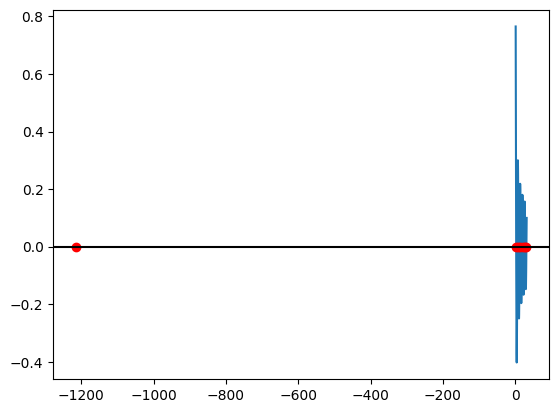
\includegraphics{Include/Images/Thesis/Documentation/NonLinear/IQI Example 2.png}
    \caption{IQI Example 2}
    \label{fig:IQI Example 2}
\end{figure}
}

\subsection{Brentt-Dekker}
Multiple implementations with small differences exist, we opted for the original one publish by Brent \cite{brent2002algorithms}, the reason behind the naming of Brent-Dekker Algorithm is because at first Dekker in conjunction with Wingartenn and their respective colleagues proposed an initial version, later Brent came an offer a better approach and convergence \cite{Press2007}, in some references like Scipy's they will call this algorithm Brent-Wingartenn-Dekker Algorithm.


\begin{algorithm}[H] 
\DontPrintSemicolon 
\SetKwInOut{Input}{Input}
\SetKwInOut{Output}{Output} 
\SetKwProg{Fn}{Function}{}{}
\SetKwFunction{FBrentDekker}{zBrentDekker} 
\SetKw{KwRaise}{Raise}

\Input{Function $f$, interval $[a,b]$, tolerance $tol$, maximum iterations $stop_iters$, arguments $\ast args$} 
\Output{Zero of $f$ in $[a,b]$} 

\Fn{zBrentDekker($f, interval, tol, stop\_iters, iters, steps, *args$)}{
$fa \gets f(a, *args)$; $fb \gets f(b, *args)$;\\
\lIf{$fa * fb > 0$}{\KwRaise{Error(“Function has no zeros in the given interval”)}}

$c \gets a$; $fc \gets fa$;
$d \gets b - a$;
$e \gets b - a$; \\

\lIf{$abs(fc) < abs(fb)$}{ 
    $a, b, c \gets b, c, b$;
    $fa, fb, fc \gets fb, fc, fb$; 
} 
$tolerance \gets 2 * \epsilon * abs(b) + tol$; \\
$m \gets 0.5 * (c - b)$; $iterations \gets 0$; \\

\While{$abs(m) > tolerance$ \textbf{and} $fb$ \textbf{and} $iterations < stop\_iters$}{ 
\lIf{$abs(e) < tolerance$ \textbf{or} $abs(fa) <= abs(fb)$}{ 
    $d \gets m$; $\bigwedge$
    $e \gets m$; 
} 
\Else{ 
    $s \gets fb / fa$; \\
    \lIf{$a == c$}{ 
        $p \gets 2 * m * s$; $\bigwedge$
        $q \gets 1 - s$; 
    } 
    
    \Else{ 
        $q \gets fa / fc$; $r \gets fb / fc$; \\
        $p \gets s * (2 * m * q * (q - r) - (b - a) * (r - 1))$; \\
        $q \gets (q - 1) * (r - 1) * (s - 1)$; } 
        
    \lIf{$p > 0$}{ $q \gets -q$;} 
    \lElse{$p \gets -p$;} 
    
    $s \gets e$; $\bigwedge$ $e \gets d$; 
    
    \lIf{$2p < 3m\cdot q - |tolerance * q|$ and $p < abs(0.5\cdot s\cdot q)$}{ 
        $d \gets p / q$; 
       } 
    \lElse{ $d \gets m$; $e \gets m$; } 
} 

$a \gets b$; $\bigwedge$ $fa \gets fb$;\\ 
$b \gets b + d$ \textbf{if} $abs(d) > tolerance$ \textbf{else} $b + np.sign(m) * tolerance$; \\
$fb \gets f(b, *args)$; \\
\lIf{$np.sign(fb) == np.sign(fc)$}{ 
    $c, fc, d, e \gets a, fa, b - a, b - a$ 
} 
\lElseIf{$abs(fc) < abs(fb)$}{ 
    $a, b, c \gets b, c, b$; $fa, fb, fc \gets fb, fc, fb$ 
} 
$tolerance \gets 2 * \epsilon * abs(b) + tol$; \\
$m \gets 0.5 * (c - b)$; $iterations \gets iterations + 1$ 
} 
$zero \gets b$\\
\Return $zero$\;}


\caption{Brent-Dekker's Algorithm}

\label{algo:zBrentDekker} 
\end{algorithm}
\subsubsection{BNumMet Examples}
\paragraph{Example 1}{
\begin{lstlisting}[language=Python]
from BNumMet.NonLinear import zBrentDekker
fun = lambda x: x**2 - 2
interval = [1, 2]
sol, nIter = zBrentDekker(fun, interval, iters = True)
print("Brent-Dekker method: x = %f, nIter = %d" % (sol, nIter))

>> Brent-Dekker method: x = 1.414214, nIter = 7
\end{lstlisting}
}
\paragraph{Example 2}{
\begin{lstlisting}[language=Python]
f = lambda x: sp.jv(0, x) # Bessel function of the first kind of order 0
interval = lambda n: [n * np.pi, (n + 1) * np.pi] # Interval for the n-th zero

zeros = [ zBrentDekker(f, interval(n)) for n in range(0, 10)]


x = np.arange(1, 10 * np.pi, np.pi / 50)
y = f(x)
plt.plot(x, y)
plt.plot(zeros, np.zeros(len(zeros)), "ro")
plt.axhline(0, color="k")
plt.show()
\end{lstlisting}
\begin{figure}[H]
    \centering
    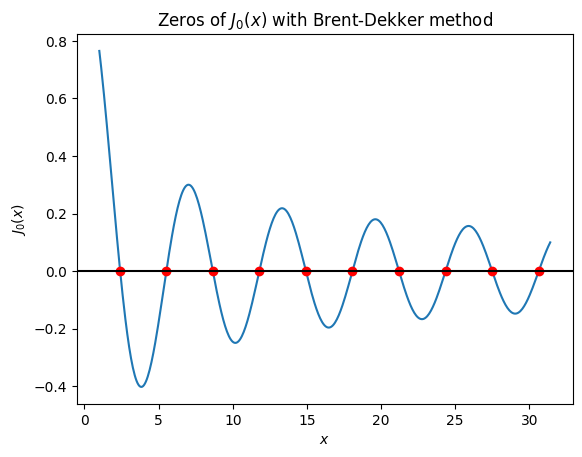
\includegraphics{Include/Images/Thesis/Documentation/NonLinear/Brentt-Dekker Example 2.png}
    \caption{Brentt-Dekker Example 2}
    \label{fig:Brentt-Dekker Example 2}
\end{figure}
}